\section{引言}
\label{sec:introduction}

本文的研究对象为非中心对称钡--钇--锌硅酸盐$\mathrm{Ba_5Y_{12}Zn[O(SiO_4)]_8}$。研究目标包括三方面：确认目标相的组成与结构归属；厘清可重复获得该相的相形成条件；判断含Zn相与无Zn四方Ba--Y硅酸盐之间是否存在连续的组成--结构关系。原始报道在开放体系中以高温溶液法生长晶体，并由单晶X射线衍射（SCXRD）确定结构\cite{ababaikeri2024ba5y12zn}。该结构兼具高配位稀土--氧骨架和孤立或复合硅酸根单元，可为复杂硅酸盐的结构组装和非中心对称氧化物的组成设计提供参照。

目标相的直接报道仅明确了晶体的存在及其结构，尚未给出可独立复现的投料组成、相形成范围或块体相纯样品的制备方法\cite{ababaikeri2024ba5y12zn}。因此，本文不由结构相关化合物的条件组合出一条“最佳配方”，而是区分单晶生长、固相反应和相图筛查各自能够解决的问题，并据此设计可区分不同结构假设的实验。全文保留文献中的数值及其限制条件；结构相关体系与工艺参照体系仅用于提出实验参照。

\subsection{相关体系的研究现状}

\paragraph{Ba--Y--Si--O四方硅酸盐系列。}
早期助熔剂法生长实验将$\mathrm{Ba_{5+x}Y_{13}Si_8O_{41}}$报道为伴生晶相；随后的151组BaO--K$_2$O--Y$_2$O$_3$--SiO$_2$--MoO$_3$体系实验表明，Y$_2$O$_3$\slash SiO$_2$比、MoO$_3$用量和冷却速率共同影响硅酸盐的结构类型与晶体质量\cite{kolitsch2009crystal,wierzbickawieczorek2017high}。现代单晶研究将相关名义组成重新审定为非化学计量$\mathrm{Ba_xY_{26}Si_{16}O_{71+x}}$；陶瓷实验还表明，玛瑙研磨可能引入SiO$_2$，使块体样品偏离名义配比\cite{yamane2024synthesis,yamane2024microstructure}。另一项相区研究结合能谱（EDS）、连续旋转电子衍射（cRED）、同步辐射粉末X射线衍射（PXRD）和中子衍射确认了$\mathrm{Ba_5Y_{13}[SiO_4]_8O_{8.5}}$，并观察到竞争相和玻璃区\cite{gulay2024navigation}。上述结果表明，目标相附近是由Ba\slash Y\slash Si比、氧计量、液相组成和热历史共同控制的相区，而非一条孤立的配方。

\paragraph{Ba--Zn--Si--O结构相关化合物。}
Ba$M$SiO$_4$（$M$~=~Co、Zn、Mg）属于填充鳞石英（stuffed-tridymite）衍生结构族，表明二价四面体阳离子可在特定骨架中相互取代，但不能据此认为其结构与含Y目标相同构\cite{liu1993structures}。BaZn$_2$Si$_2$O$_7$的低温结构与高温结构可由中子衍射和X射线衍射区分，表明观测温度和冷却路径会影响结构判定\cite{lin1999phase}。BaZnSi$_3$O$_8$的固相反应研究则依次经煅烧、压片、烧结和受控冷却，并以同步辐射或实验室X射线衍射表征\cite{zou2021crystal}。因此，Ba--Zn--Si--O体系文献的主要启示在于同时记录Zn源、气氛、冷却路径以及高温和室温下的相组成，而非直接移用某一温度。

\paragraph{Y--Si--O工艺参照体系。}
Y$_2$SiO$_5$和Y$_2$Si$_2$O$_7$均存在多种多晶型，已通过高温溶液法、熔体法和提拉法（Czochralski法）制备。衍射、局域谱学和高温表征表明，不同多晶型及冷却后的产物须分别鉴定\cite{redhammer2003beta,becerro2004revisiting,dolan2008structures,pang2005study}。这些工作有助于规范坩埚、助熔剂、挥发损失、缓冷和退火等条件的记录，但不能证明$\mathrm{Ba_5Y_{12}Zn[O(SiO_4)]_8}$适用于同样的生长方法。

\subsection{本文结构}

本文首先核对目标相及相关结构的文献出处，其次总结前人实验对组成、竞争相、污染和热历史的认识，然后比较不同合成路线及其实验条件，最后提出局部相图、Zn--Y--氧计量耦合、固相反应与高温溶液法并行以及Mg\slash Co类比四个研究方向。文中的两步无机逆合成模型仅生成待验证的前驱体集合；温度、气氛、坩埚和表征方法仍依据文献和材料化学约束确定。

图~\ref{fig:research-roadmap}\CJKecglue{}概括了本文的论证路线：相关体系先用于确定结构关系、竞争相和工艺边界；相图与电荷平衡分析提出候选组成，逆合成模型据此给出前驱体集合；固相反应与高温溶液法晶体生长分别检验块体相区和单晶结构；再根据相组成、实际化学计量和结构精修结果逐轮调整组成与工艺。每轮实验均应至少排除一种结构或相区假设，而非追求未经验证的“最佳配方”。

\begin{figure*}[t]
  \centering
  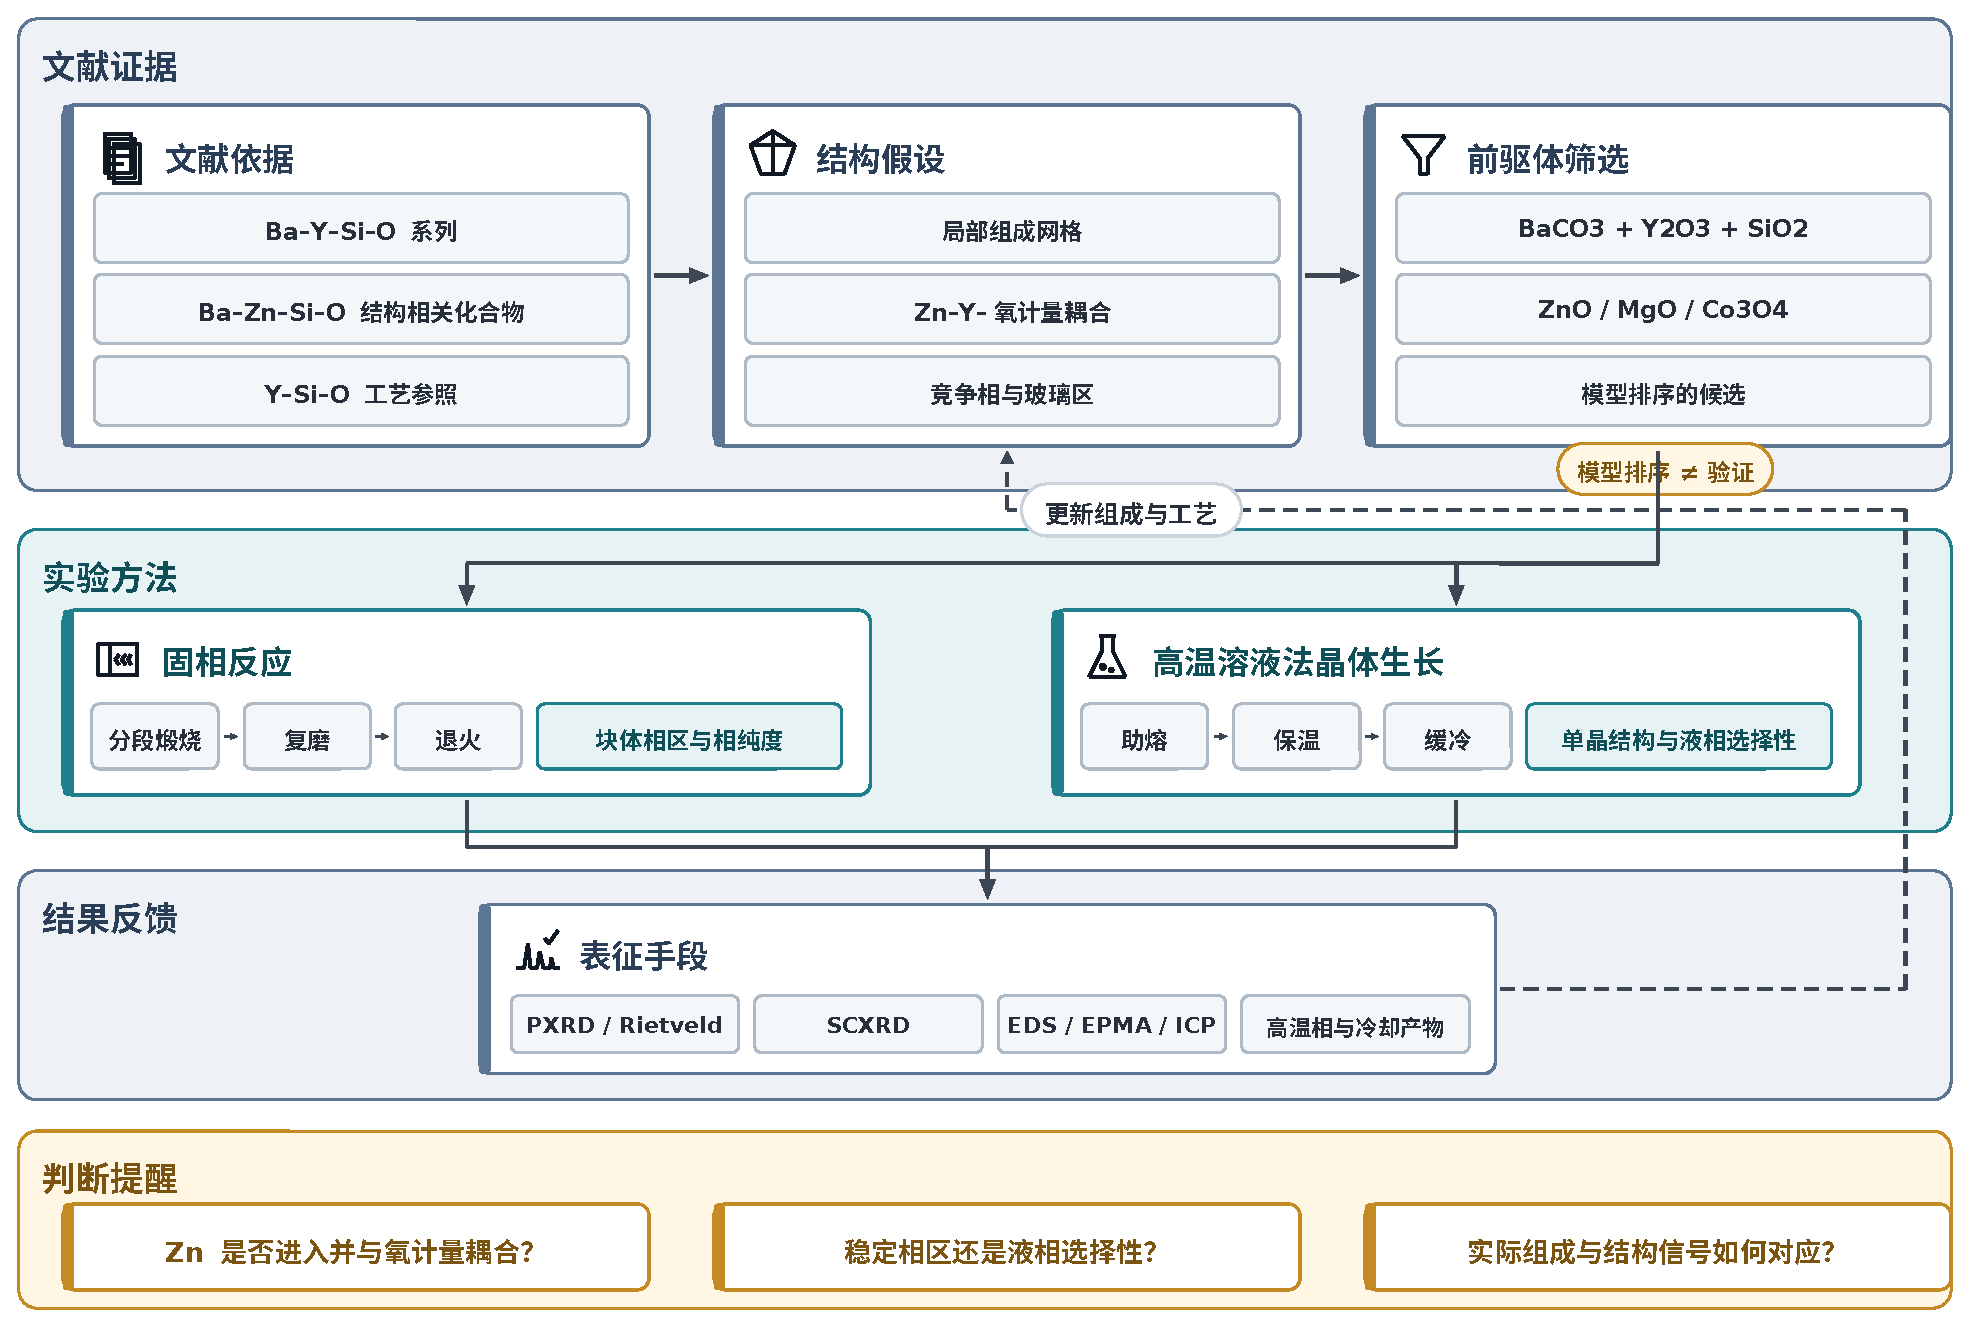
\includegraphics[width=\textwidth]{../figures/pdf/fig03_research_roadmap.pdf}
  \caption{\textbf{本文的研究路线。}Ba--Y--Si--O、Ba--Zn--Si--O和Y--Si--O体系先用于确定结构关系、竞争相和工艺边界；相图与电荷平衡分析提出候选组成，两步无机逆合成模型给出前驱体集合；固相反应与高温溶液法晶体生长分别考察块体相区和单晶结构，表征结果用于调整后续的组成和工艺。}
  \label{fig:research-roadmap}
\end{figure*}
